%Katerina Muskova (xmusko00)
%2019, Duben

\documentclass[11pt, a4paper]{article}
\usepackage[left=2cm,text={17cm, 24cm},top={3cm}]{geometry}

\usepackage[czech]{babel}
\usepackage[utf8]{inputenc}
\usepackage[T1]{fontenc}
\usepackage{times}

\usepackage{blindtext}
\usepackage{hyperref}
\usepackage{csquotes}

\usepackage{multirow}
\usepackage[ruled,vlined,czech,linesnumbered,noline,longend]{algorithm2e}
%\usepackage[ruled,czech,linesnumbered,longend,noline]{algorithm2e}
\usepackage{algorithmic}
\usepackage{graphics}
\usepackage{picture}
\usepackage{epsf}
\usepackage{epstopdf}
\usepackage{pdflscape}


%\usepackage{amsmath, amsthm, amssymb, amsfonts, bm}
%\usepackage{mathtools}

\begin{document}

%%%%%%%%%%%%%%%%%%%%%%%%%%%%%%% TITLE %%%%%%%%%%%%%%%%%%%%%%
\begin{titlepage}

\begin{center}
	\Huge \textsc{Vysoké učení technické v~Brně}\\
	\huge \textsc{Fakulta informačních technologií}\\
		
	\vspace{\stretch{0.382}}
	\huge Typografie a publikování\,--\,3. projekt\\
	\Huge Tabulky a obrázky
	\vspace{\stretch{0.618}}
\end{center}

{\Large \today \hfill Kateřina Mušková}
\end{titlepage}

%%%%%%%%%%%%%%%%%%%%%%%%%%%%%%% DOCUMENT %%%%%%%%%%%%%%%%%%%

\section{Úvodní strana}
Název práce umístěte do zlatého řezu a nezapomeňte uvést dnešní datum a vaše jméno a příjmení

\section{Tabulky}
Pro sázení tabulek můžeme použít buď prostředí \verb|tabbing| nebo prostředí \verb|tabular|.

\subsection{Prostředí \texttt{tabbing}}
Při použítí \verb|tabbing| vypadá tabulka následovně:

\begin{tabbing}
    Vodní melouny \qquad \= Cena \qquad \= Množství \kill
    \textbf{Ovoce} \>
    \textbf{Cena} \>
    \textbf{Množství} \\
    Jablka \> 25,90 \> 3\,\,kg \\
    Hrušky \> 27,40 \> 2,5\,\,kg\\
    Vodní melouny \> 35,-- \> 1\,\,kus \\
\end{tabbing}

Toto prostředí se dá také použít pro sázení algoritmů, ovšem vhodnější je použít prostředí \verb|algorithm| nebo \verb|algorithm2e| (viz sekce \ref{sec:Al}).   
   
\subsection{Prostředí tabular}
Další možností, jak vytvořit tabulku, je použít prostředí \verb|tabular|. Tabulky pak budou vypadat takto\footnote{Kdyby byl problém s~\texttt{cline}, zkuste se podívat třeba sem: http://www.abclinuxu.cz/tex/poradna/show/325037.}.

\begin{table}[ht]
	\catcode`\-=12
	\begin{center}
	\begin{tabular}{| l | r | r |} \hline
						& \multicolumn{2}{|c|}{\textbf{Cena}} \\ \cline{2-3} 
		\textbf{Měna} 	& \textbf{nákup} 	& \textbf{prodej} \\ \hline
		EUR 			& 25,615			& 27,20 \\
		GBP 			& 29,899			& 31,80 \\
		USD 			& 22,571 			& 25,51 \\ \hline
	\end{tabular}
	\caption{Tabulka kurzů k~dnešnímu dni} \label{tbl1}
	\end{center}
\end{table}


\begin{table}[h]
	\begin{center}
	\catcode`\-=12
	\begin{tabular}{|c|c|}
		\hline
		$A$			& $\neg A$ \\ \hline
		\textbf{P} 	& N  \\ \hline
		\textbf{O} 	& O~\\ \hline
		\textbf{X} 	& X  \\ \hline
		\textbf{N} 	& P  \\ \hline
	\end{tabular}
 	%%%%%%%%%%%% new tblr
	\begin{tabular}{|c|c|c|c|c|c|} \hline
		\multicolumn{2}{|c|}{\multirow{2}{*}{$A \wedge B$} } & \multicolumn{4}{|c|}{$B$}\\ \cline{3-6}
		\multicolumn{2}{|c|}{} &\textbf{P}	&\textbf{O}	&\textbf{X}	&\textbf{N} \\ \hline
		\multirow[c]{3}{*}{$A$}&\textbf{P}	&P 			&O 			&X			&N \\ \cline{2-6}
							   &\textbf{O}	&O 			&O 			&N			&N \\ \cline{2-6}
							   &\textbf{X}	&X 			&N 			&X			&N \\ \cline{2-6}
							   &\textbf{N}	&N 			&N 			&N			&N \\ \hline		
	\end{tabular}
	%%%%%%%%%%%% new tblr
	\begin{tabular}{|c|c|c|c|c|c|} \hline
		\multicolumn{2}{|c|}{\multirow{2}{*}{$A \vee B$} } & \multicolumn{4}{|c|}{$B$}\\ \cline{3-6}
		\multicolumn{2}{|c|}{} &\textbf{P}	&\textbf{O}	&\textbf{X}	&\textbf{N} \\ \hline
		\multirow[c]{3}{*}{$A$}&\textbf{P}	&P 			&P 			&P			&P \\ \cline{2-6}
							   &\textbf{O}	&P 			&O 			&P			&O \\ \cline{2-6}
							   &\textbf{X}	&P 			&P 			&X			&X \\ \cline{2-6}
							   &\textbf{N}	&P 			&O 			&X			&N \\ \hline		
	\end{tabular}
	%%%%%%%%%%%% new tblr
	\begin{tabular}{|c|c|c|c|c|c|} \hline
		\multicolumn{2}{|c|}{\multirow{2}{*}{$A \vee B$} } & \multicolumn{4}{|c|}{$B$}\\ \cline{3-6}
		\multicolumn{2}{|c|}{} &\textbf{P}	&\textbf{O}	&\textbf{X}	&\textbf{N} \\ \hline
		\multirow[c]{3}{*}{$A$}&\textbf{P}	&P 			&O 			&X			&N \\ \cline{2-6}
							   &\textbf{O}	&P 			&O 			&P			&O \\ \cline{2-6}
							   &\textbf{X}	&P 			&P 			&X			&X \\ \cline{2-6}
							   &\textbf{N}	&P 			&P 			&P			&P 	 \\ \hline		
	\end{tabular}
	%%%%%%%%%%%% tab end
	\caption{Protože Kleeneho trojhodnotová logika už je \uv{zastaralá}, uvádíme si zde přílad čtyřhodnotové logiky} \label{tbl2}
	\end{center}
\end{table}

\section{Algoritmy} \label{sec:Al}
Pokud budeme chtít vysázet algoritmus, můžeme použít prostředí \verb|algorithm|
\footnote{Pro nápovědu, jak zacházet s~prostředím \texttt{algorithm}, můžeme zkusit tuhle stránku: \\ http://ftp.cstug.cz/pub/tex/CTAN/macros/latex/contrib/algorithms/algorithms.pdf.}
 nebo \verb|algorithm2e|
\footnote{Pro \texttt{algorithm2e} zase tuhle: http://ftp.cstug.cz/pub/tex/CTAN/macros/latex/contrib/algorithm2e/doc/algorithm2e.pdf.}.
 Příklad použití prostředí \verb|algorithm2e| viz Algoritmus \ref{alg}.

\begin{algorithm}[h]
\caption{\textsc{Fast}SLAM} \label{alg}

\SetKwInOut{Input}{Input}\SetKwInOut{Output}{Output}
\Input{$(X_{t-1}, u_t, z_t)$}
\Output{$X_t$}

\SetNlSty{}{}{:  } % dvojtecka za cisly radku
\SetInd{1em}{1em}
\SetNlSkip{-1.33em}

	\begin{algorithmic}[1]
		\STATE $\overline{X_t} = X_t = 0$
		\FOR{$k = 1$ to $M$}
		\STATE $x^{[k]}_{t} = sample\_motion\_mode(u_t ,x^{[k]}_{t-1})$
		\STATE $\omega^{[k]}_{t} = measurement\_model(z_t ,x^{[k]}_{t}, m_{t-1})$
		\STATE $m^{[k]}_{t} = updated\_occupancy\_grid(z_t ,x^{[k]}_{t}, m_{t-1}^{[k]})$
		\STATE $\overline{X_t} = \overline{X_t} + \langle x^{[m]}_{x}, \omega^{[m]}_{t} \rangle$
		\ENDFOR
		\FOR{$k = 1$ to $M$}
		\STATE $\textnormal{draw } i \textnormal{ with probability} \approx \omega^{[i]}_{t}$
		\STATE $\textnormal{add } \langle x^{[k]}_{x}, m^{[k]}_{t} \rangle \textnormal{ to } X_t$
		\ENDFOR
		\RETURN $X_t$
	\end{algorithmic}
\end{algorithm}

\section{Obrázky}
Do našich článků můžeme samozřejmě vkládat obrázky. Pokud je obrázkem fotografie, můžeme klidně použít bitmapový soubor. Pokud by to ale mělo být nějaké schéma nebo něco podobného, je dobrým zvykem takovýto obrázek vytvořit vektorově.

\begin{figure}[h]
	\begin{center}
	\scalebox{0.4}{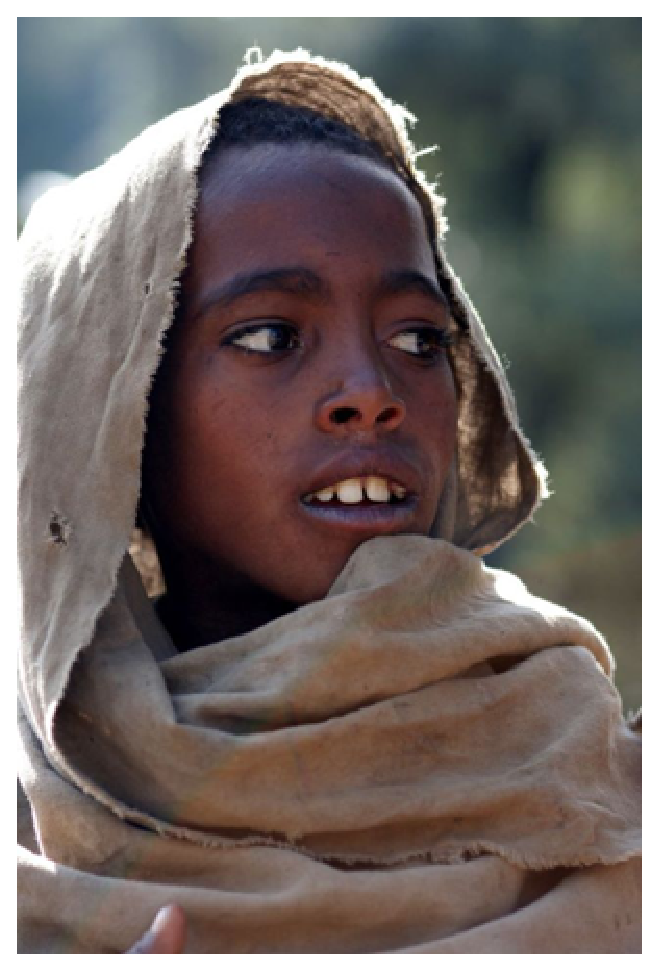
\includegraphics{obr/etiopan.eps}
        \reflectbox{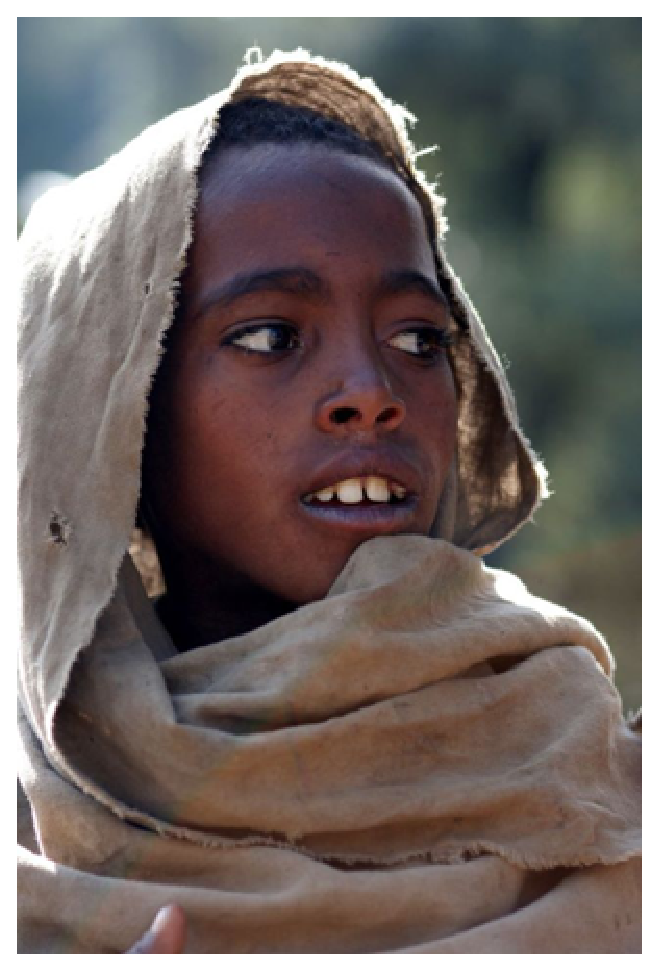
\includegraphics{obr/etiopan.eps}}}
	\caption{Malý Etiopánek a jeho bratříček} \label{obr1}
	\end{center}
\end{figure}

\newpage

Rozdíl mezi vektorovým\,\dots
\begin{figure}[ht]
	\begin{center}
	\scalebox{0.4}{
\includegraphics{obr/oniisan.eps}}
	\caption{Vektorový obrázek} \label{obr2}
	\end{center}
\end{figure}

\dots\,a bitmapovým obrázkem

\begin{figure}[ht]
	\begin{center}
	\scalebox{0.6}{
\includegraphics{obr/oniisan2.eps}}
	\caption{Bitmapový obrázek} \label{obr3}
	\end{center}
\end{figure}


se projeví například při zvětšení.

Odkazy (nejen ty) na obrázky \ref{obr1}, \ref{obr2} a \ref{obr3}, na tabulky \ref{tbl1} a \ref{tbl2} a také na algoritmus \ref{alg} jsou udělány pomocí křížových odkazů. Pak je ovšem potřeba zdrojový soubor přeložit dvakrát.

Vektorové obrázky lze vytvořit i přímo v~\LaTeX u, napřílad pomocí prostředí \verb|picture|.


\begin{landscape}
\begin{figure}[h]
	\begin{center}
	
	\setlength{\unitlength}{0,2cm}
	\begin{picture}(130,70)(0,0)
	
		\put(0,0){\framebox(130,70)}
		\put(20, 60){\circle{10}}
		
		%strecha
		\linethickness{0.8pt}
		\put(10,50){\line(1,0){102}}
		\put(10,50){\line(0,-1){10}}
		\put(112,50){\line(0,-1){15}}
		\put(10,40){\line(1,0){10}}
		\put(112,35){\line(-1,0){12}}
		
		% 1. blok
		\put(20,43){\line(1,0){17}}
		\put(20,43){\line(0,-1){39}}
		\put(37,43){\line(0,-1){5}}
		\put(37,30){\line(0,-1){26}}
		
			\put(27,30){\framebox(30,8)}
			\multiput(20,20)(0,1){8} {\line(1,0){17}}
			\multiput(20,20)(0,1){8} {\framebox(4,4)}
		
		% 2. blok
		\put(30,43){\line(0,1){2}}	
		\put(30,45){\line(1,0){70}}	
		\put(60,45){\line(0,-1){41}}
		
		% 3. blok
			\put(60,15){\framebox(2,20)}
			\put(62,17){\framebox(2,14)}
			\put(64,19){\framebox(2,8)}	
		\put(100,45){\line(0,-1){24}}	
		
		% trojuhelnik
		\put(86,35){\line(1,-1){31}}	
		\put(86,35){\line(0,-1){31}}		
		
			
		
		\linethickness{5pt}
		\put(12,4){\line(1,0){106}}
	
	\end{picture}
	\end{center}
	\caption{Vektorový obrázek modernío bydlení vhodného pro 21. století.}	
\end{figure}
\end{landscape}

\end{document}
